    \section{Specificatie}
    Het spel, \emph{Grudge of the Oblivious} (\textsc{goto}), dat wij van plan zijn om te ontwerpen, is een combinatie van een FPS spel en een RTS spel. Dit betekent dat de gebruiker van het spel zowel kan schieten als gebouwen kan bouwen. Het spel speelt zich af in een oorlog tussen twee rivaliserende robot-bendes. Deze robot-bendes hebben een corresponderend commandocentrum. In het spel kan een robot-bende als team gezien worden, een dergelijk team bestaat uit meerdere robots en spelers. Elke speler bestuurt \'e\'en robot. Er zijn evenveel robots als spelers.

    Het doel van het spel is om het commandocentrum van de tegenstander te vernietigen. De spelers hebben lasergeweren om de tegenstanders dood te schieten en torens aan te vallen. Torens kunnen door spelers worden neergezet op het terrein. Deze torens kosten goud om te bouwen. De spelers verdienen goud in een gezamenlijke kas door mijnen te bouwen over delfplaatsen. Verder kan goud worden verdiend door tegenstanders te doden en hun torens te vernietigen. Als een speler dood gaat of een toren kapot gaat, zal deze een muntje achterlaten dat vervolgens door alle spelers kan worden opgepakt. Wij richten ons met dit spel voornamelijk op jongeren van 14 tot 25 jaar.

    Hier beschrijven we alleen de noodzakelijke onderdelen van het spel. Een lijst van mogelijke uitbreidingen is toegevoegd in appendix \ref{app:optioneel}.

	\subsection{Terrein}
    Het terrein kan in wezen allerlei vormen hebben, we leggen hier slechts twee simpele restricties op. Allereerst moet het terrein eerlijk zijn: dit betekent dat een team geen voordeel mag hebben vanwege de kaart. We eisen bovendien dat de kaart rechthoekig is.

    Op het terrein zijn twee commandocentra geplaatst, voor beide teams een commandocentrum. Het kan gewenst zijn dat elk team bij de start van het spel ook al een aantal extra torens heeft ter bescherming van het commandocentrum. Over het terrein zijn een aantal delfplaatsen verdeeld. Andere obstakels mogen aanwezig zijn, maar zijn niet noodzakelijkerwijs aanwezig. Alle objecten met uitzondering van spelers worden geplaatst op een rooster. In figuur \ref{fig:map1} en \ref{fig:map2} zijn twee mogelijke beginconfiguraties van het spel getoond.

    \begin{figure}[h]
        \begin{subfigure}{0.5\linewidth}
            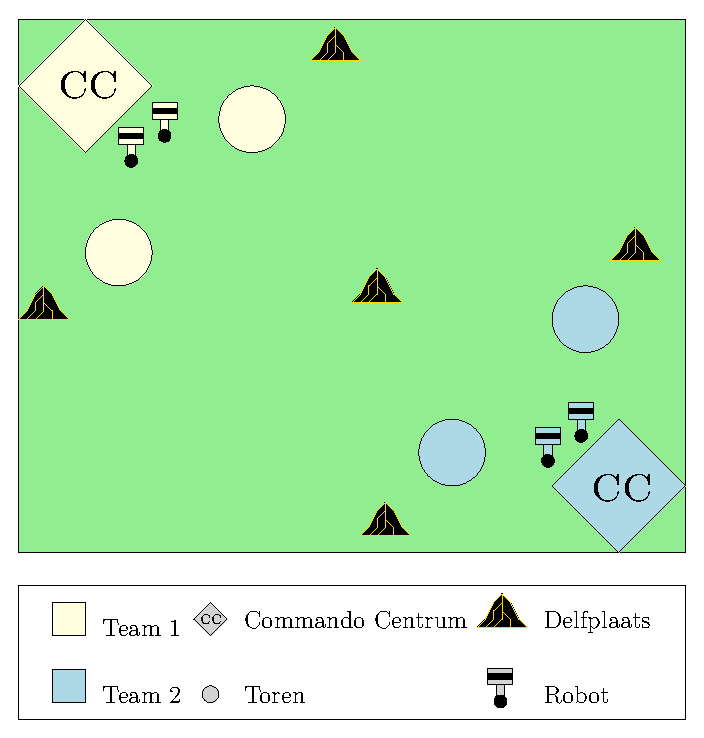
\includegraphics[width=\textwidth]{../Graphics/Map1.eps}
            \caption{Een bijna vierkant terrein met vier spelers}
            \label{fig:map1}
        \end{subfigure}\hspace{10mm}
        \begin{subfigure}{0.5\textwidth}
                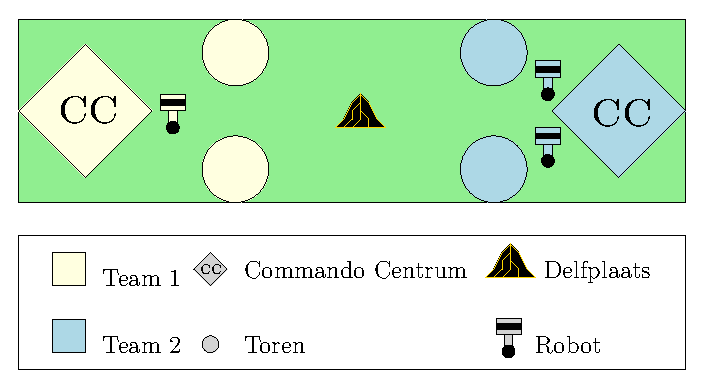
\includegraphics[width=\textwidth]{../Graphics/Map2.eps}
                \caption{Een breed terrein met drie spelers}
                \label{fig:map2}
        \end{subfigure}
        \caption{Twee verschillende beginconfiguraties van het spel}
    \end{figure}

    \subsection{Spelers}
    Een speler behoort tot \'e\'en van beide teams, spelers van een bepaald team zijn te identificeren door kleuren. De speler ziet de wereld vanuit de positie van zijn robot. Men kan de kijkrichting aanpassen, zodat deze elke willekeurige richting kan zijn. Als de kijkrichting verder naar links of rechts wordt gedraaid, draait de robot mee. De speler heeft een lasergeweer waarmee hij op andere spelers en torens kan schieten om deze te vernietigen. Het lasergeweer schiet laserstralen met een `oneindige' snelheid in de huidige kijkrichting. Bij het begin van het spel heeft de robot nog een volledig harnas. Zodra de speler wordt geraakt, wordt de conditie van het harnas slechter. Het is echter niet mogelijk dat een speler het harnas van een andere speler uit hetzelfde team beschadigt.
    \FloatBarrier
    Een speler gaat dood als zijn harnas kapot is. In dat geval zal hij na een bepaalde hoeveelheid tijd terugkeren bij het commandocentrum met een volledig harnas. Ook kan een speler gebouwen bouwen, hiervoor gebruikt hij goud uit de kas van het team. De spelers kunnen op het grondvlak bewegen met een vaste snelheid in elke richting. De enige voorwaarde hierbij is dat de spelers op de kaart blijven en niet door een gebouw lopen. Het is dus wel mogelijk dat spelers door elkaar heen kunnen lopen. De speler kijkt vanuit een derde persoon perspectief. In een derde persoon perspectief wordt de sc\`ene bekeken vanaf een punt vlak achter de speler. Het is eventueel mogelijk om dit verder uit te breiden, zodat de speler kan wisselen van derde persoon perspectief naar eerste persoon perspectief.

    \subsection{Gebouwen}
    Er zijn drie soorten gebouwen: torens, mijnen en commandocentra. Torens schieten op spelers en andere gebouwen in hun bereik. Mijnen kunnen over delfplaatsen worden gebouwd met het doel de inkomsten van een team te vergroten. In principe levert elke mijn een vaste hoeveelheid goud voor de gezamenlijke kas op. Deze hoeveelheid wordt periodiek toegevoegd aan de kas.

    Uit sommige delfplaatsen kan maar een bepaalde hoeveelheid goud worden gehaald, daarna is de delfplaats op. Dan zal de mijn over die delfplaats geen verdere bijdrage meer leveren voor de gezamenlijke kas. We staan echter ook delfplaatsen toe die een onbeperkte hoeveelheid goud bevatten. Standaard levert elke mijn hetzelfde bedrag op met dezelfde periode, maar dit kan later nog worden aangepast.

    Het commandocentrum is het belangrijkste gebouw van het team. Als dit gebouw kapot is, heeft het bijbehorende team verloren. Gebouwen kunnen door spelers worden beschoten, waardoor deze worden beschadigd. Gebouwen kunnen op geen enkele mogelijke manier hersteld worden. Optioneel zou men mechanismen in het spel kunnen toevoegen om deze gebouwen te herstellen. Alle gebouwen behoren tot \'e\'en van beide teams, deze gebouwen kunnen weer ge\"identificeerd worden door de kleur van het gebouw.

    \subsection{Verzamelbare voorwerpen}
    Er is maar \'e\'en verzamelbaar voorwerp: een muntje. E\'en of meerdere muntjes worden achtergelaten door spelers die dood gaan en torens die worden vernietigd. Een muntje heeft een bepaalde waarde in goud. De waarde van de muntjes zijn proportioneel aan de gezamenlijke kas van het team waarvan de speler is doodgegaan. Als een toren is vernietigd, dan is de waarde van de muntjes proportioneel aan de kosten van de toren. De waarde van de muntjes moet echter altijd kleiner zijn dan de kosten van de toren. Gedurende een spel moeten deze proporties vast zijn.

    Als een speler doodgaat, wordt bovendien nog de waarde van de muntjes afgetrokken van de gezamenlijke kas van die speler. Een muntje kan vervolgens opgepakt worden door alle spelers. Het muntje is dus het voedsel element in ons spel. De waarde van het muntje zal dan toegevoegd worden aan de kas van het bijbehorende team.

    \subsection{Initialisatie}
    De spelers kunnen zelf kiezen bij welk team ze gaan, onder de voorwaarde dat elk team minstens \'e\'en speler heeft. Bij de start van het spel staan alle spelers bij het commandocentrum. Zoals al eerder gezegd, hebben alle spelers dan nog een volledig harnas. Bovendien heeft elk team een zekere positieve hoeveelheid goud in de gezamenlijke kas, die voor beide teams natuurlijk gelijk moet zijn. Er kunnen minstens twee mijnen gebouwd worden met deze hoeveelheid goud.
    \FloatBarrier

    \subsection{Gebruikersomgeving}
    \label{sec:UI}

    Via de gebruikersomgeving kan de speler de interactie met het 3D-model aangaan. De volgende componenten worden weergegeven op de gebruikersomgeving tijdens het spel:
    \begin{itemize}
    \item De hoeveelheid goud van het team, deze hoeveelheid staat achter een goudstaaf.
    \item De sterkte van het harnas, die wordt weergegeven door middel van een statusbalk.
    \item Het vizier van de speler.
    \end{itemize}

    We plaatsen het vizier van de speler altijd in het midden van het scherm. Hierdoor weet de speler dus in welke richting wordt geschoten. De speler wordt altijd iets links van dit vizier getekend. Voor de duidelijkheid hebben wij hier ook een figuur van gemaakt. Een plattegrond van de kaart wordt ook aangegeven in figuur \ref{fig:UI}. De plattegrond is een extra optie in het spel.
    \begin{figure}[H]
    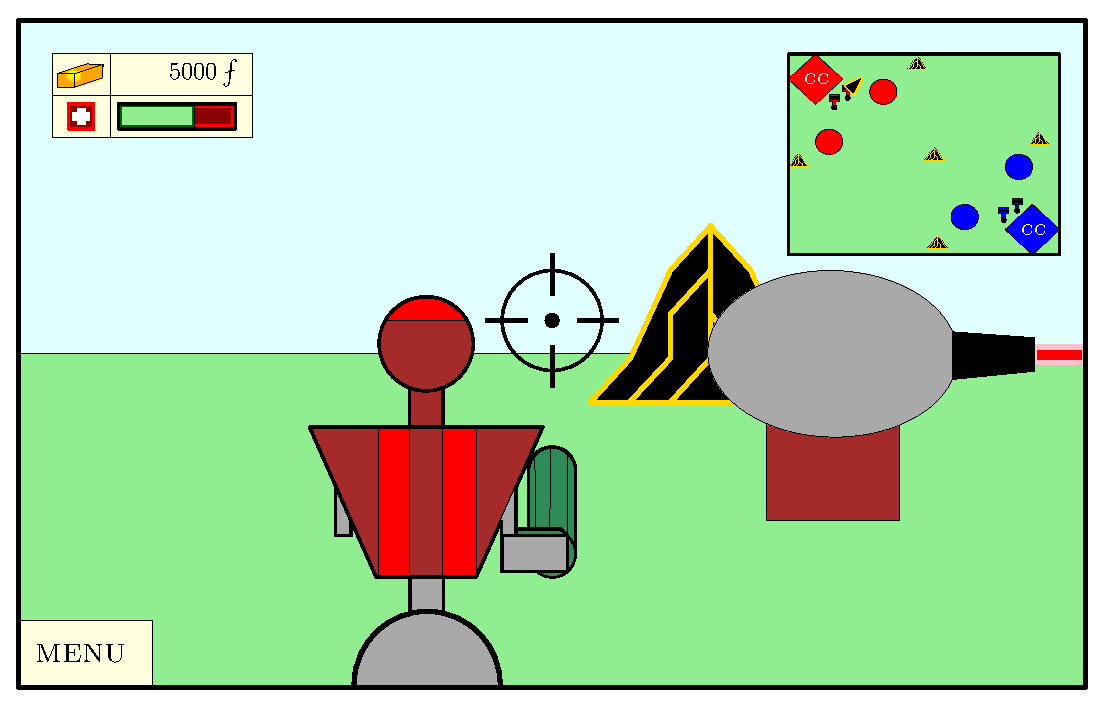
\includegraphics[width=0.9\textwidth]{../Graphics/UI.eps}
    \caption{De gebruikersomgeving tijdens het spel}
    \label{fig:UI}
    \end{figure}
    De besturing van de robot kan met de \textsc{wasd}-toetsencombinatie of door gebruik te maken van de pijltjes-toetsen. Hiervoor geven we de volgende tabel:
    \begin{table}[H]
        \small
        \centering
        \begin{tabular}{| l | l |}
        \hline
        Knop & Reactie \\ \hline
        \textsc{w} of $\uparrow$ & De robot beweegt, indien mogelijk, vooruit naar de huidige kijkrichting toe \\ \hline
        \textsc{a} of $\leftarrow$ & De robot draait naar links \\ \hline
        \textsc{s} of $\downarrow$ & De robot beweegt, indien mogelijk, achteruit van de huidige kijkrichting af \\ \hline
        \textsc{d} of $\rightarrow$ & De robot draait naar rechts \\ \hline
        \end{tabular}
        \caption{Knoppen met bijbehorende reactie}
        \label{tab:planning}
    \end{table}

    De speler kan schieten door op de muis te drukken. Een gedetailleerde beschrijving van het schieten is opgenomen in appendix \ref{app:schieten}. Door de muis naar boven of naar beneden te bewegen, kijkt de speler verder omhoog of omlaag respectievelijk. Op analoge wijze kan de speler naar links of naar rechts draaien door respectievelijk de muis naar links of naar rechts te bewegen. Merk op dat het vizier altijd in het midden van het scherm blijft. De speler ziet dit dus doordat de horizon omlaag of omhoog schuift.

    \subsection{Het neerzetten van gebouwen}
    De speler kan ook opdracht geven om op een bepaalde plek een gebouw neer te laten zetten. Om een gebouw neer te zetten moet de speler eerst op de knop \textsc{b} drukken. Dan gaat de speler in de zogenaamde \emph{bouw-modus}. Op dat moment wordt er een klein menu onderaan het scherm van de speler afgebeeld. Door middel van sneltoetsen kan de speler een gebouw van dit menu kiezen.

    Merk op dat de muis op dit moment nog steeds de kijkrichting bestuurt. Als het gebouw gekozen is, wordt op de ondergrond een rooster getekend. Door middel van het vizier kan de speler een plek op het rooster aanwijzen. De speler kan door te klikken dan de opdracht geven om het gebouw neer te laten zetten. Op dat moment wordt de bijbehorende hoeveelheid goud uit de gezamenlijke kas gehaald. Vervolgens zal het gebouw ook worden neergezet.

    Als de speler niet genoeg goud in de gezamenlijke kas heeft voor het gebouw, wordt de speler gewaarschuwd. Dan wordt er natuurlijk geen goud uit de gezamenlijke kas gehaald en het gebouw niet neergezet. Na het neerzetten van het gebouw gaat de speler weer uit de bouw-modus. Op elk moment kan dit proces afgebroken worden door op de knop \textsc{b} te drukken. Dit kan gezien worden in figuur \ref{fig:gebouw}.

    \begin{figure}
    \centering
    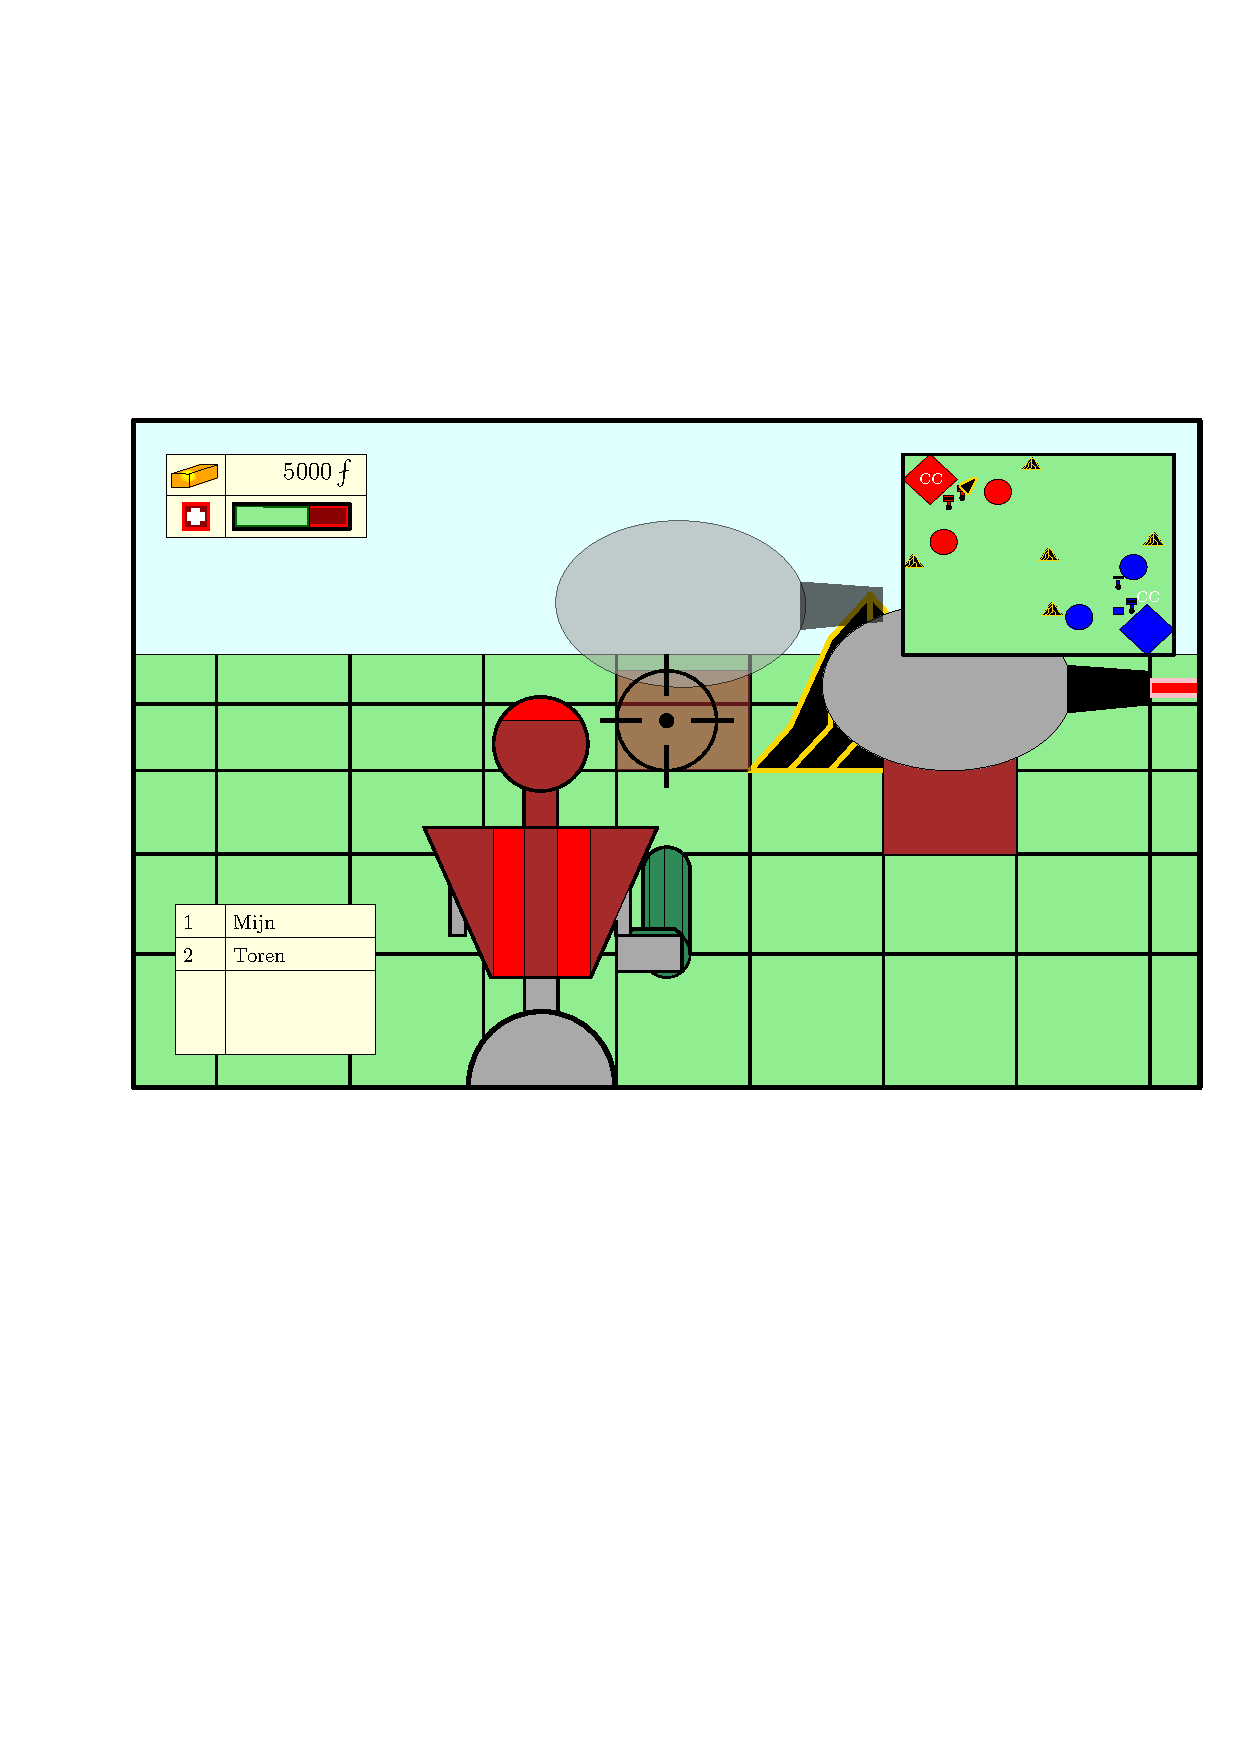
\includegraphics[width=\textwidth]{../Graphics/UI2.pdf}
    \caption{Een voorbeeld van het neerzetten van een gebouw in de gebruikersomgeving}
    \label{fig:gebouw}
    \end{figure} 